\chapter{Abstract Design}

\section{Control Topology}
While the controls topology is not a primary focus of this thesis, it is an
essential driver of the converter design.

The starting requirements in the controls design for this project was to
eliminate as many single-points of failure as possible using a separate
controller per-phase.

This approach immediately drives a few control topology decisions.  First,
typical AC drive algorithms require knowledge of the complete state of the
machine in order to generate commands.
This would either necessitate either a very fast and tightly coupled
communication structure or some method to decouple the controls from some of
the machine states.
As we are using a machine with 6 phases to allow for fault tolerance,
broadcasting current sensor information each cycle would already overwhelm a
typical CAN network.
To avoid this problem we use the dual-wye connection of the drive and have
each phase module sense only 3 currents: Its own, one on the same wye, and one
on the opposite wye.
Standard 3-phase drives already use a variant of this method by only sensing
two currents for control.
This allows a single phase controller to have a full view of the currents in
its wye while monitoring the other wye for faults.

By symmetry, running an identical control algorithm for each phase and picking
the correct voltage output will allow standard vector control concepts to be
used with minimal overhead.
The variations in input sensors however will need to be corrected for and some
effort will be required to achieve good power balance between phases.

Position sensing is also a problem and presents a single-point failure
mechanism.
For this work we are simply using a standard position sensor though standard
resolver concepts can be extended to allow for each phase module to have its
own resolver stator while using the same rotor.

For this work, we will be staring with V/Hz control as this is relatively
robust and easy to implement with limited feedback required.


\subsection{Non-synchronized PWM}
While control states may be managed between modular drive processors with only
moderate difficulty, the classical assumption that all PWM carriers are
synchronized presents significant difficulty as a delay of only a few
microseconds represents a significant phase delay.
Thankfully, at normal carrier to fundamental ratios, the phase of the PWM
carrier is unimportant to a first order as the machine inductance filters out
the high frequency switching components.
Quartz crystal-based main oscillators are quite stable and allow frequency
tolerance below 100ppm without any special calibration.
For a 20kHz PWM system, the beat frequency between PWM carriers will be at a
frequency of 2Hz.
This beat frequency will manifest as a peaking of the $\frac{dV}{dt}$ applied
to the machine windings relative to the frame every 0.5s or longer depending
on the specific spread of oscillator frequencies.
While this phenomenon has little effect on the control of the machine, the
effects on bearing currents and insulation lifetime have not been investigated.

\subsection{Fault Management}
A detailed consideration of fault management has been reserved for future work, but 

\section{DC-Link Design}
DC-link design is a topic that is often overlooked in converter design.
Usually it is relegated to rules-of-thumb which are often based on sound
reasoning, but typically end up being used in situations where the assumptions
they are based on do not hold.

The first of these rules is to size DC-Link capacitors based on a certain
capacity per Watt of converter power rating.
This rule is extremely easy to apply, but is typically based on the assumption
of DC-Link currents being dominated by the 120Hz or 180Hz current ripple of a
single-phase or 6-pulse diode rectifier.
This rule also is specific to one voltage level as the ripple current and thus
capacitance requirement is decreased as the inverse of the DC-link voltage.
If not driven by controls requirements on DC-link voltage variation, this rule
also assumes specific current handling capabilities of the capacitor
(Typically electrolytic).

The next common rule is to design based on an allowed voltage ripple.
This rule is significantly more robust than the converter-power based rule
above as it takes into account varying ripple current conditions.
This rule is also often dictated by the controls design as control accuracy
will suffer if the DC-Link voltage variation is not decoupled.

A final rule of thumb is to size the DC-link capacitance to be thermally rated
for a ripple current that is a given fraction of the converter's rated output
current (typically two thirds the RMS phase current for common 3-phase
converters).
This is a very robust rule in terms of managing component lifetime, but may
cause excess DC-Link voltage ripple if polymer film-based capacitors are used
due to their excellent current handling capability even at low capacitance
ratings.

The matter of the precise spectrum of DC-link current is treated well in
\cite{McGrath09} where the current from a switching converter is calculated by
convolving the output current with the switching voltage waveform.
This approach confirms the two-thirds sizing rule for conventional three-phase
2-level VSI converters and adds the insight of how specific frequency
components are related between phases.

Fig. \ref{fig3phCur} shows how the RMS ripple current is effected by changes
in both modulation index and the output power factor of a three-phase
converter.
This plot is delineated as a ratio of RMS phase current to RMS DC-link ripple.
The worst-case is at approximately a 0.6 modulation index with unity power
factor (either motoring or generating).
This plot also clearly shows that it is the switches, not the DC-link
capacitor that circulates energy when a converter is operating at low power
factor.

\begin{figure}[htbp]
\centering
\label{fig3phCur}
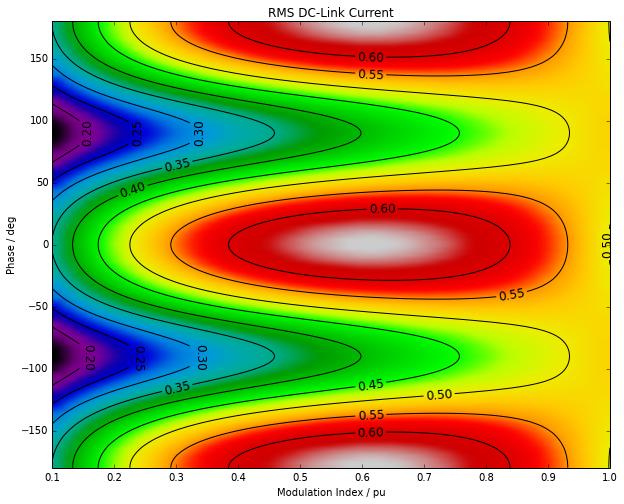
\includegraphics[width=\textwidth]{DC3phRipple}
\caption{DC-link ripple current for a three-phase, two-level VSI operating
without higher harmonic injection.  Contour lines delineate ratio of RMS phase
current to RMS ripple current.}
\end{figure}

The main takeaway from this is that the interconnect between phases should
have lower impedance than the interconnect between any single phase and the
DC-source in order to allow cancellation of modulation-referenced ripple while
the capacitors must be sized to handle switching-referenced ripple.

These three rules all encapsulate both their driving assumptions the two
actual drivers of DC-link design.

First, whatever design is chosen must be capable of handling ripple-related
thermal loads.
This is a function of both dielectric heating effects and joule
losses in capacitors and inductors.
As capacitor technology advances with
improvements in film capacitors and upcoming dielectric materials such as
glass, designs based on thermal capability will become more necessary.

Second, a DC-link structure is at its core an impedance matching component
which must present a low impedance to the power converter's switching pole
at the switching frequency and higher, must present a low impedance at twice
the power frequency due to reactive power handling requirements, and must
present a high impedance at DC in order to ensure that bulk power flow comes
from the power source.

While this is typically handled with bulk capacitance for standard VSI-based
designs, the size and temperature constraints of the integrated modular motor
drive require a more creative hybrid approach.
An interesting aside is that resonant-link converters fully exploit this
requirement to reduce switching losses and reactive component size.

\subsection{Interconnect Design}
For the integrated modular motor drive, we cannot tolerate the low temperature
ratings of electrolytic capacitors.
Because of this limitation, the total bulk capacitance available is much lower
than would typically be used in a converter of this size.
Furthermore, due to the distributed nature of the converter, reactive power
currents must be passed through the DC-link structure to other modules before
returning to the machine.
In order to maintain an effective low impedance at the power frequency for
reactive power while shielding these currents from the power source, a
star-and-ring topology was chosen as described in previous work on IMMD power
electronics.

While this ring-and-star approach is very effective at handling
power-frequency harmonics, it does not keep a stiff DC-link at the switching
frequency and higher.
In order to accomplish this, I chose a frequency-splitting technique similar
to what is used in high performance logic decoupling.
To this end, the DC-link capacitance is split into three parts on each module:
A bulk polyproylene film capacitor, a pair of multilayer ceramic capacitors,
and an integrated PCB capacitor.

The overall DC-link layout is shown in Fig. \ref{figInverterLayout}.

\begin{figure}[htbp]
	\centering
	\label{figInverterLayout}
	\includegraphics[width=\textwidth]{\detokenize{power_inverter}}
	\caption{Schematic showing interconnection of power inverter and
	machine.}
\end{figure}

\subsection{Capacitor Sizing}
Capacitor sizing was based entirely on current handling capability and size
constraints.
As power-frequency components are being primarily handled by the DC-Link
interconnect we require little capacitance to manage reactive power flow.
For the bulk DC-link capacitance, a 700V 20$\mu F$ film capacitor from TDK was
chosen as it can handle nearly the entire ripple current of a phase at rated
load.
This capacitor will be absorbing the kHz range ripple from the converter
switching.
The ceramic capacitors were chosen for high-voltage, low-inductance, and low
dielectric loss.
As these capacitors are placed directly on the DC terminals of the power
modules, they will be handling the MHz range power frequencies caused by
switching edges.
Finally, the PCB itself was designed with nearly uniterrupted power planes
which provided each board with 1nF of somewhat lossy capacitance at very low
inductance which ensured that >10MHz ripple would not be injected into the
other capacitors.

This multi-layer design allowed for low impedance with reduced overall
capacitor size as is shown in the results section.


\section{Peak Ratings}
Electric machine and drive system ratings are influenced by a variety of
factors.
While continuous ratings for rated operating conditions are well defined and
easily modeled and tested, peak ratings are dependent on definitions.
The determination of peak ratings is further complicated by marketing
influences in that a large "peak power" number is an easily quoted figure of
merit even if it has little real-world backing.

The peak rating of an electric drive system is driven by a number of factors
depending on the peak time required.
For peak times on the order of one electrical cycle, the power limit is driven
by the saturation current allowed by the power switches and the
demagnetization limit of the permanent magnets in the electric machine.
Both of these limits are effected by the starting temperature of the
electrical drive system, but are largely independent of other thermal effects
as the peak time is too short.

For the FreedomCar/USDrive specification, peak power rating is defined as an
83\% overload for 18 seconds.
This overload time is of the same order as machine thermal time constants.
From a converter sizing standpoint, this overload rating requires that the
power switches are capable of handling the full overload power as they have
sub-second thermal time consents.
The remainder of the converter design however only needs to be rated to the
continuous load as capacitor and interconnect thermal time constants are
measured in minutes or longer.
The cooling system for the power converter must be able to handle
approximately the same overload as the machine as the extra cooling load from
the power semiconductors will increase in proportion to output power.
Finally, sensing must be able to accommodate the full overload if control is to
be maintained during overloaded conditions.
